\subsubsection{Support Vector Machines (SVM) Analysis}
\label{subsubsec:discussion-svm}

SVMs performed well on both the hepatitis and the mushroom datasets,
achieving peak accuracy and F1 scores which match the best results from KNN.

A key advantage of the SVM over KNN is that SVMs are much faster during consultation time. As seen in \autoref{fig:model_comparison_mushroom},
SVMs tend to have much lower test times than KNN. This is expecially noticable for large datasets like the mushroom dataset.

\begin{figure}
    \centering
    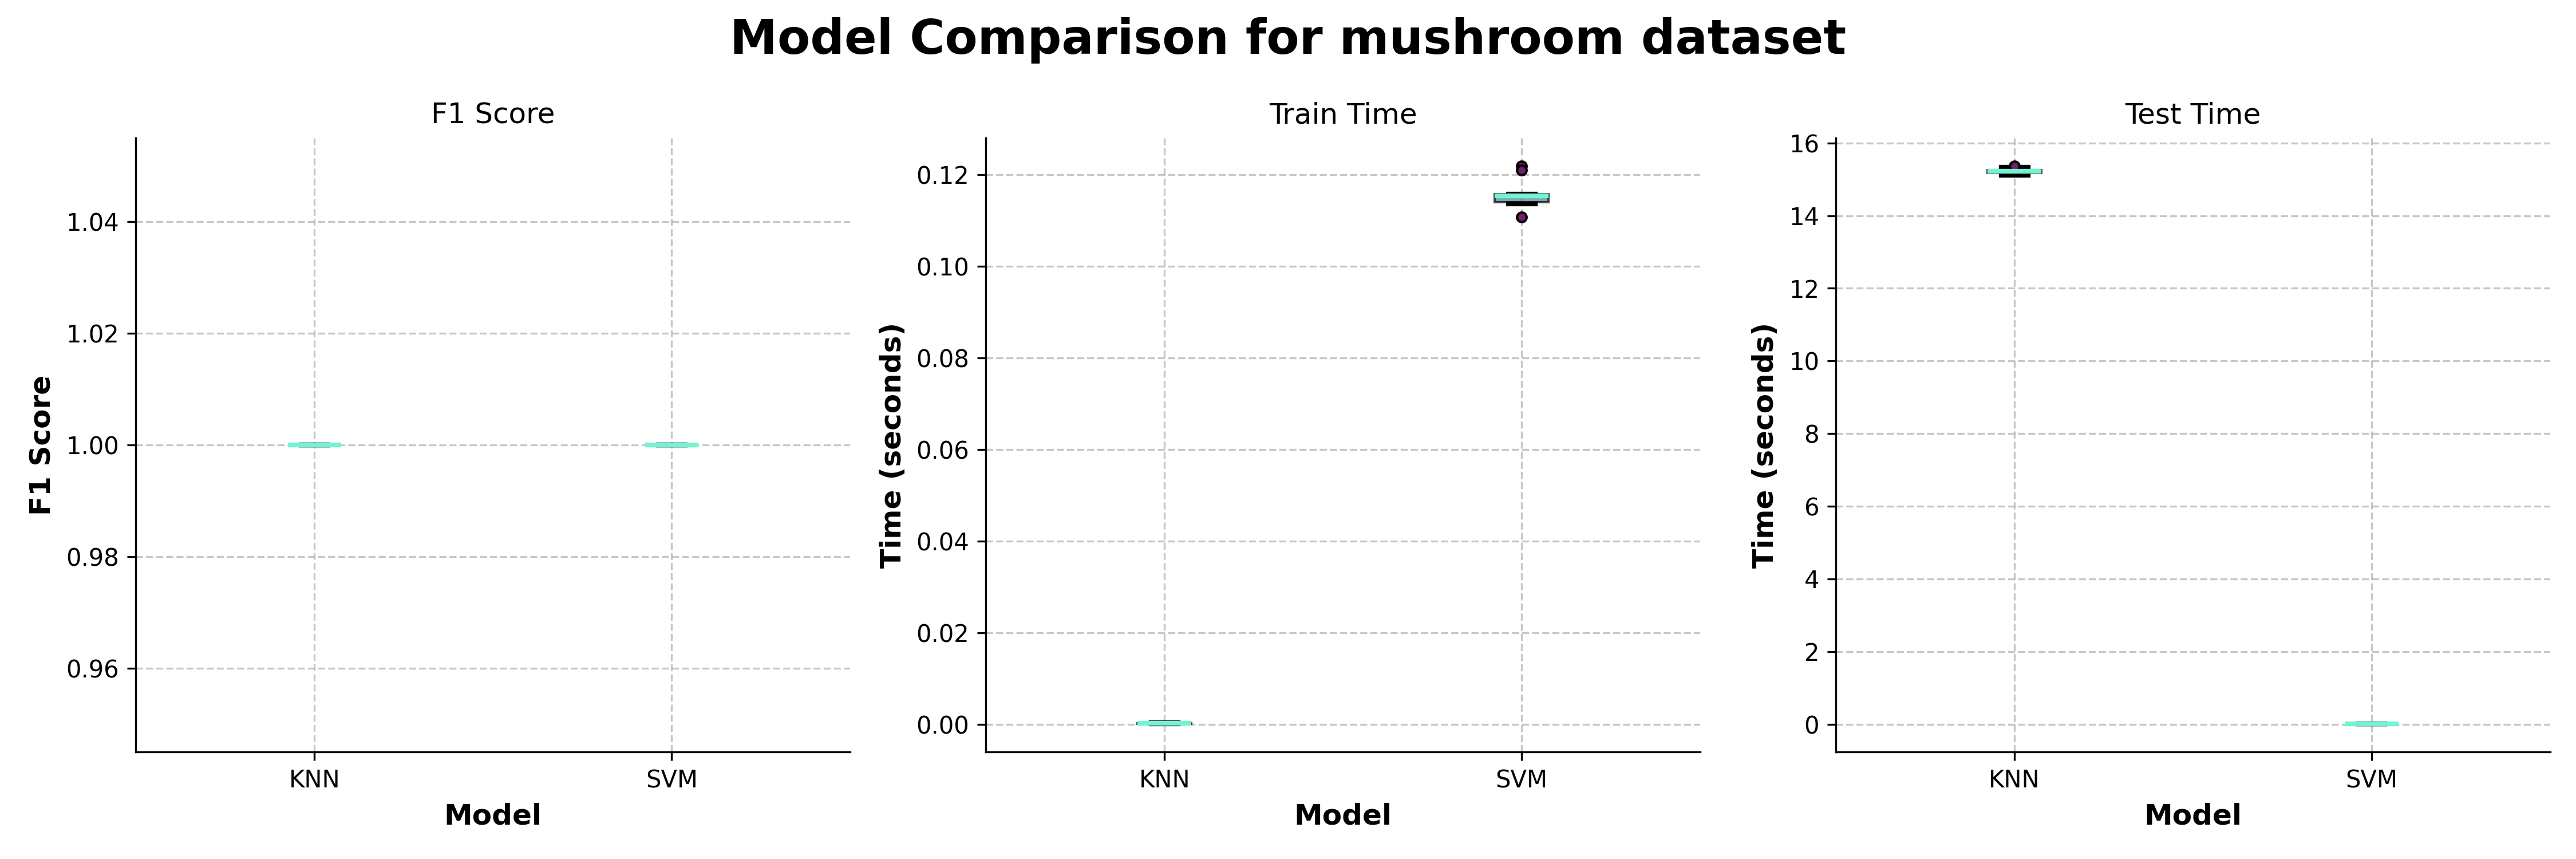
\includegraphics[width=0.9\textwidth]{figures/model_comparison_mushroom.png}
    \caption{SVM and KNN Comparison}
    \label{fig:model_comparison_mushroom}
\end{figure}


\subsubsection*{Hyperparameter Comparison}

For both the hepatitis and mushroom datasets, the configuration using the \textbf{RBF} kernel and $C=7$
achieved outstanding accuracy and F1 scores. However, because of the simple predictability
of the mushroom data, the simple \textbf{Polynomial} kernel performed just as well when used with $C=1$.
(See \autoref{tab:svm_results_hepatitis} and \autoref{tab:svm_results_mushroom}).

To compare the performance across model configurations, we employed statistical analysis methods
(see \autoref{sec:statistical-analysis}) to determine whether the various configurations showed
statistically significant differences in performance.

\begin{figure}
    \centering
    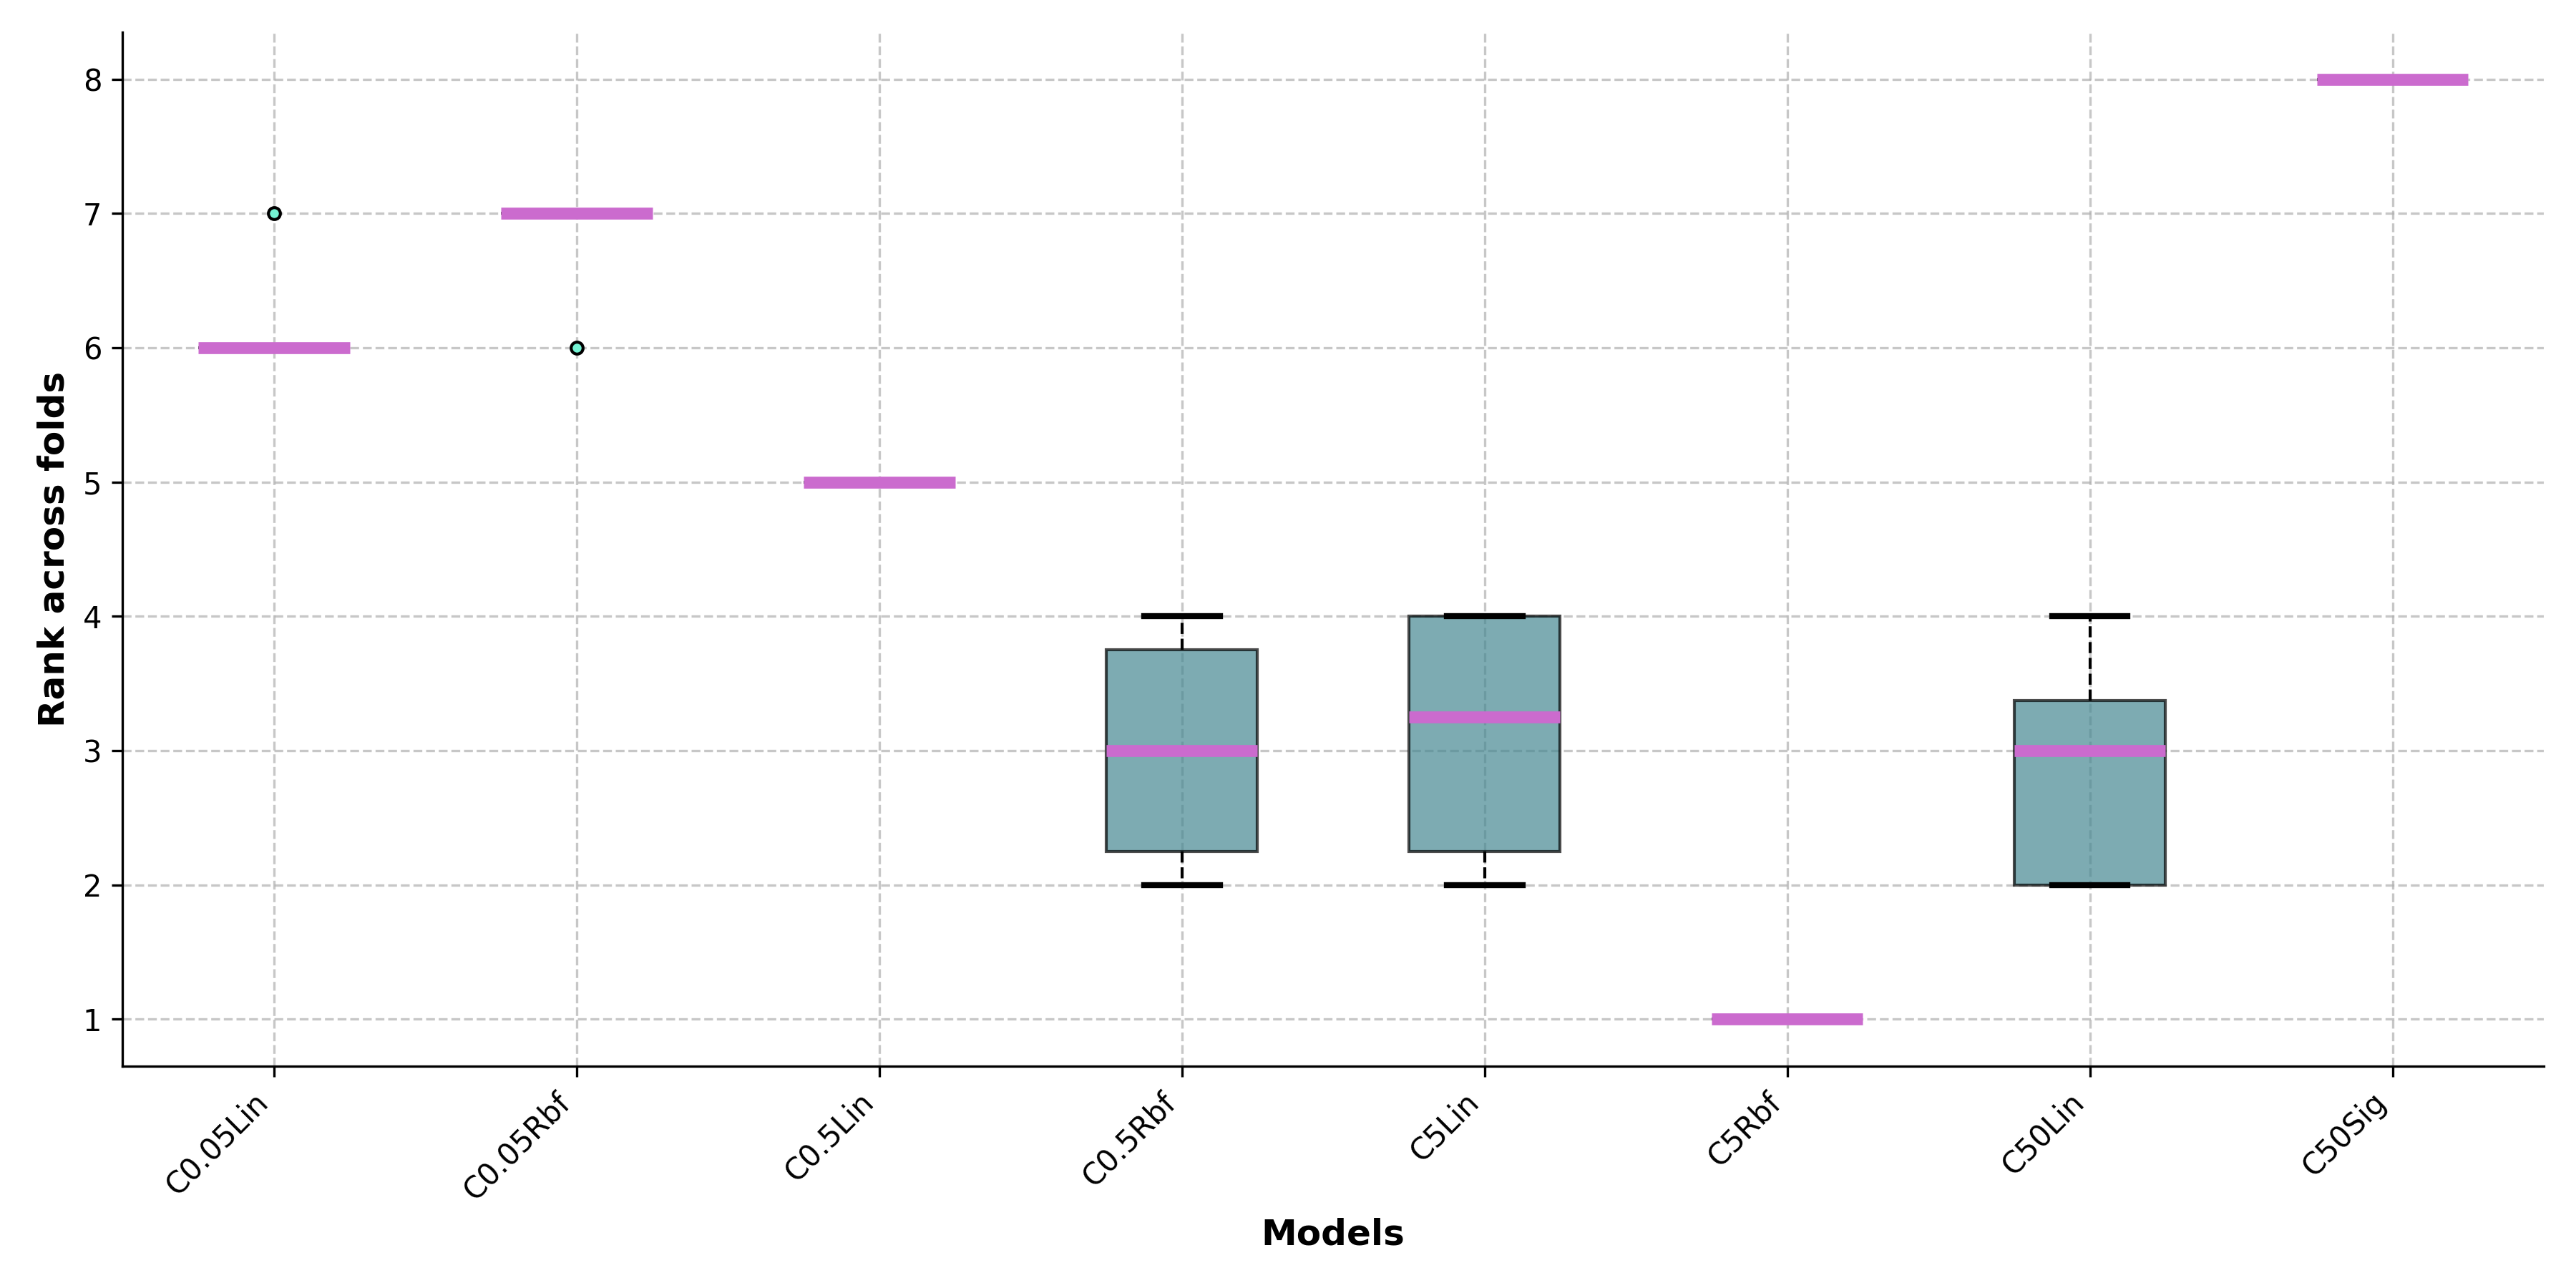
\includegraphics[width=0.9\textwidth]{figures/ranked_folds_SVM_mushroom.png}
    \caption{SVM Ranked Folds for Mushroom Dataset}
    \label{fig:ranked_folds_svm_mushroom}
\end{figure}

\begin{figure}
    \centering
    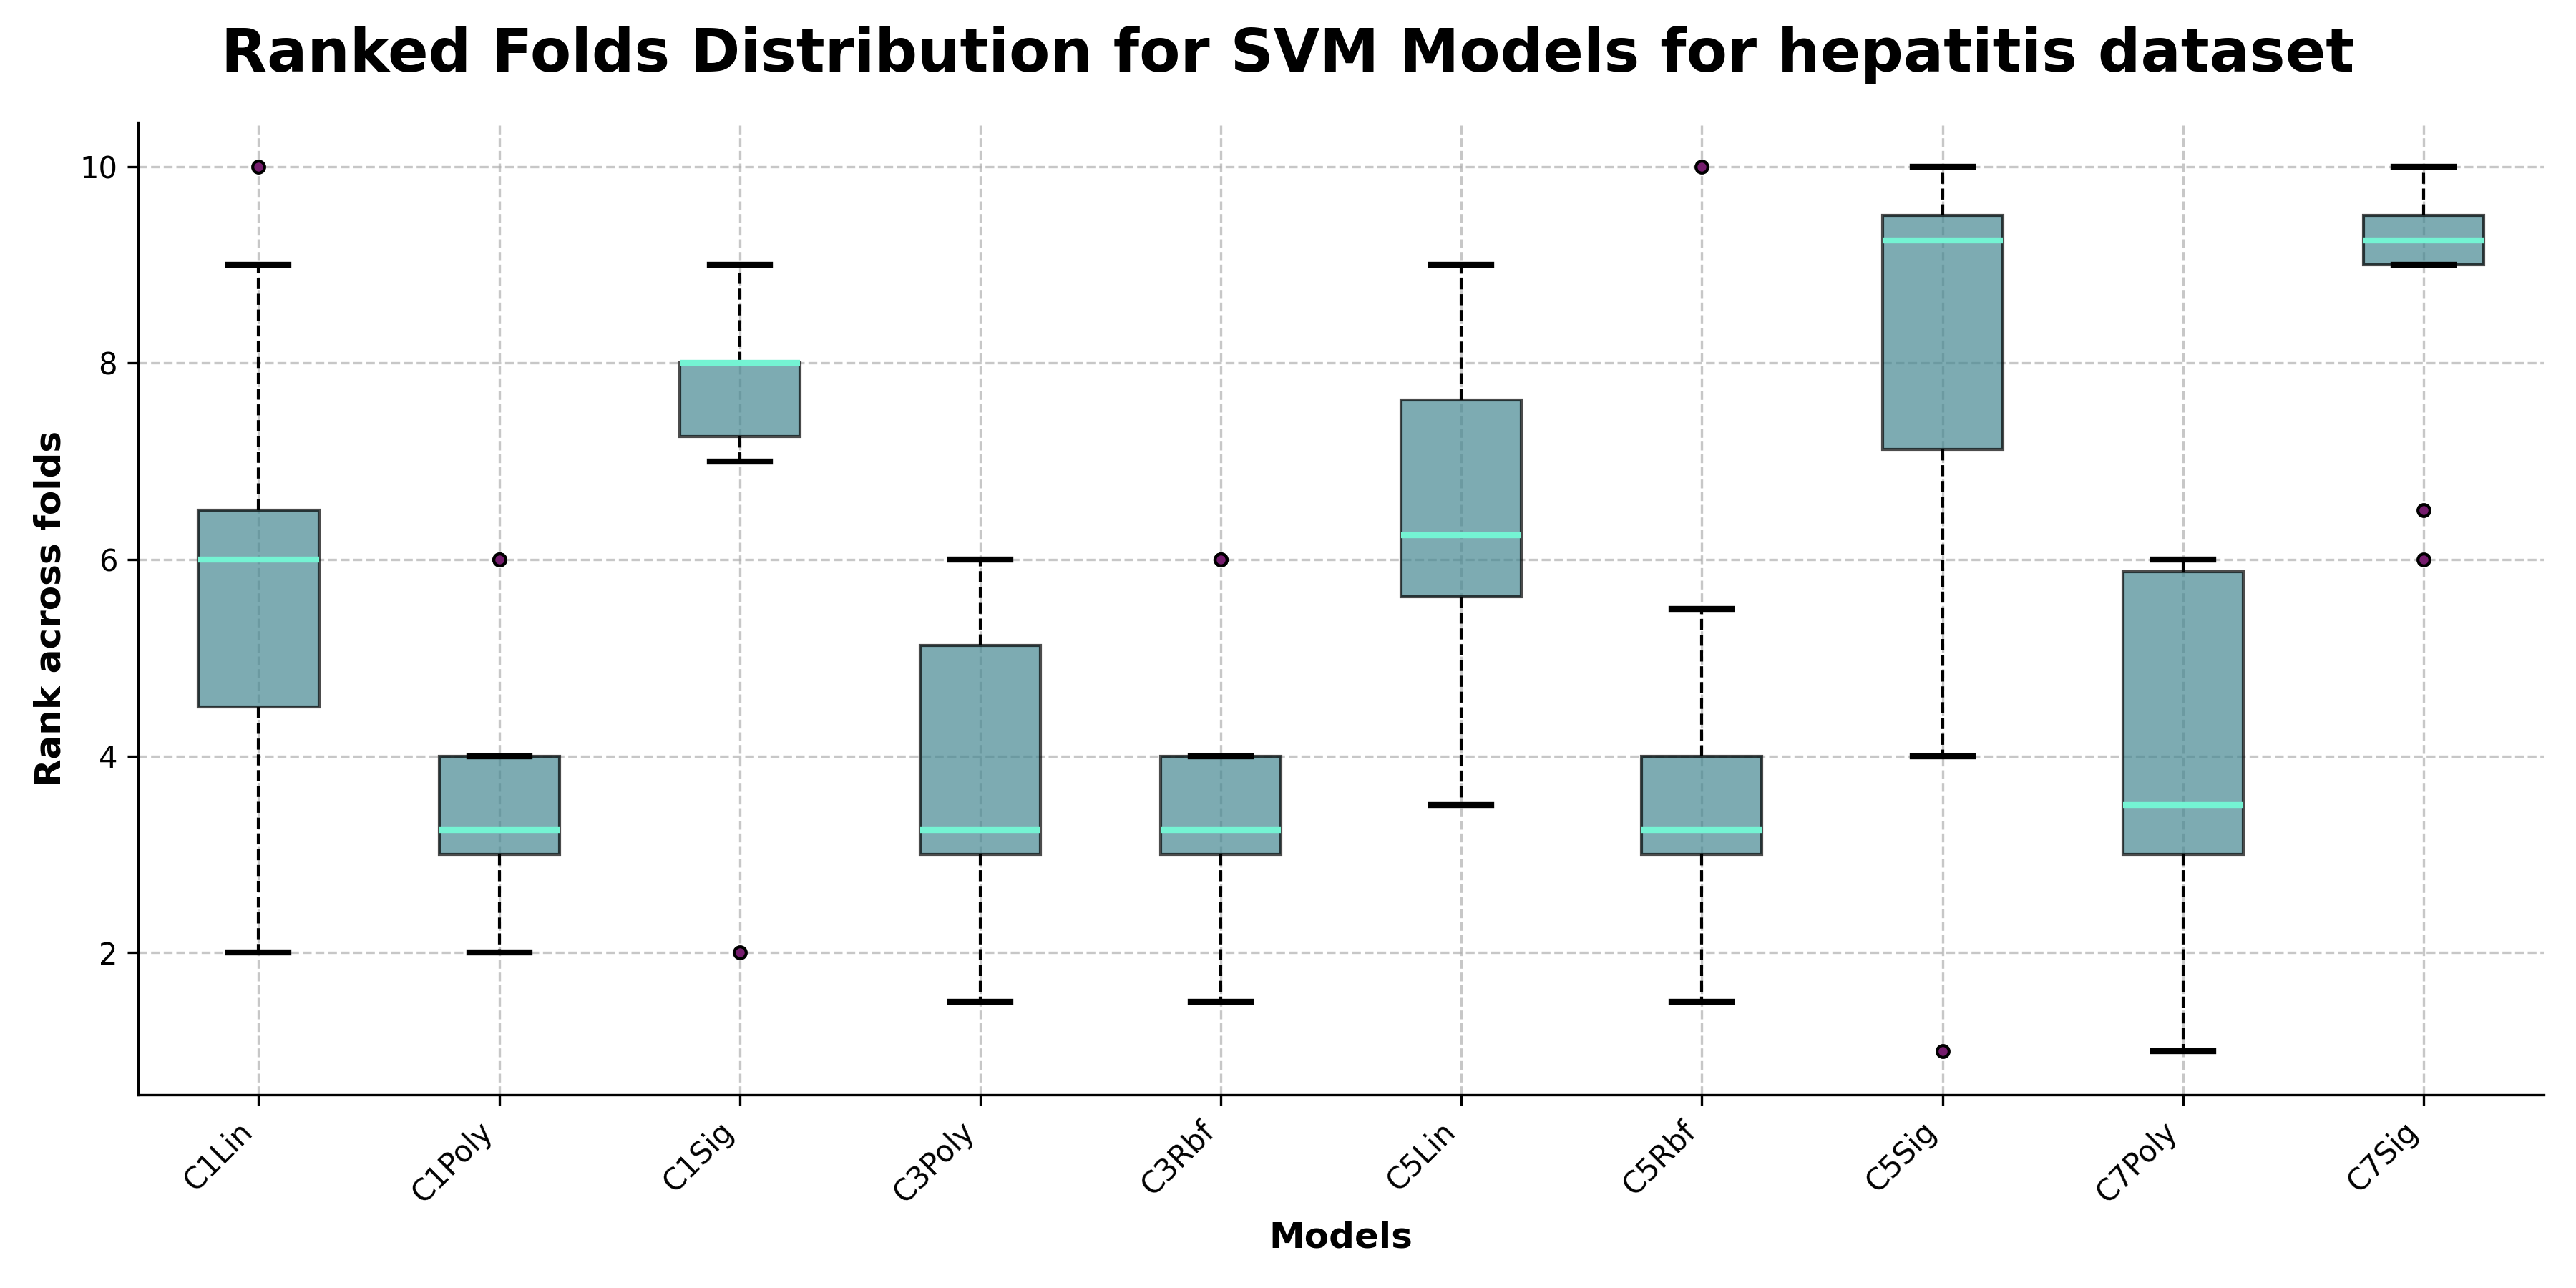
\includegraphics[width=0.9\textwidth]{figures/ranked_folds_SVM_hepatitis.png}
    \caption{SVM Ranked Folds for Hepatitis Dataset}
    \label{fig:ranked_folds_svm_hepatitis}
\end{figure}

As seen in \autoref{fig:ranked_folds_svm_hepatitis}, some models achieved 

